\documentclass[10pt]{article}
\usepackage[margin=0.8in]{geometry}
\usepackage{graphicx}
\usepackage{booktabs}
\usepackage{array}
\usepackage{longtable}
\usepackage{amsmath}
\usepackage{microtype}
\usepackage{float}
\usepackage[hidelinks]{hyperref}
\title{Supplementary Material for\\From Mechanism Activation to Forecast Value}
\author{}
\date{}
\begin{document}
\maketitle

\section{Purpose and scope}

This supplement preserves the study-level detail behind the synthesis. It does not pool task-specific scores. Each figure is copied from the corresponding returned evidence archive. The figures are descriptive mechanism and factorial diagnostics; the numeric tables and dated inference in the main paper determine the claims.

\section{Evidence inventory}

\begin{longtable}{p{1.6cm}p{2.3cm}rp{7.5cm}}
\toprule
Study & Run identifier & Fits & Preserved evidence \\
\midrule
C3R & RUN-20260929-082738-C3R & 33 & Source and data hashes; checkpoints; dated RankIC; paired and factorial inference; coalition and intervention diagnostics. \\
DARC & RUN-20260929-120135-DARC & 18 & Source and data hashes; checkpoints; frozen forecast streams; eight readouts; paired, factorial, and economic diagnostics. \\
CARE & RUN-20260930-064205-CARE & 24 & Source and data hashes; quantile predictions; calibration metrics; paired and factorial inference; analog and routing diagnostics. \\
MOSAIC & RUN-20261002-123004-MOSAIC & 21 & Source and data hashes; variance forecasts; paired and factorial inference; branch, stress, and exposure diagnostics. \\
DASH-V & RUN-20261002-151054-DASHV & 15 & Source and data hashes; frozen forecasts; delayed replay; paired and factorial inference; pooling and memory diagnostics. \\
\bottomrule
\end{longtable}

\section{Mechanism-to-claim register}

The five systems expose different internal objects, so a common diagnostic
cannot be imposed by name alone. Table~\ref{tab:claim-register} records the
observable used to establish activation, the matched counterfactual used to
test incremental value, and the principal empirical bottleneck. This mapping
prevents a mechanism plot from being interpreted as a performance comparison.

\begin{table}[H]
\centering
\small
\caption{Claim map for the five mechanisms. ``Activation'' identifies an internal change; ``matched test'' identifies the forecast-level counterfactual.}
\label{tab:claim-register}
\begin{tabular}{p{1.35cm}p{4.0cm}p{4.1cm}p{4.2cm}}
\toprule
Study & Activation evidence & Matched forecast test & Main diagnostic bottleneck \\
\midrule
C3R & Message energy, coalition inclusion, and routing entropy & Full communication-and-risk router versus the plain and risk-only cells & Candidate risks were compressed and routing remained diffuse \\
DARC & Forecast disagreement, pairwise corrections, and gate adoption & Pair-specific arbitration and gating versus global or fixed readouts & Local pair decisions did not reliably improve the completed ranking \\
CARE & Different analog sets, memory disagreement, and route entropy & Dual-memory tail route versus single-memory and dual-plain routes & Retrieval changed representations without consistent pinball-loss gain \\
MOSAIC & Nonzero downside and market-stress branch outputs & Two-branch full model versus anchor-only and one-branch cells & Corrections improved a weak anchor family but not strong controls \\
DASH-V & Time-varying pool forecasts, local reliability, and memory weights & Hierarchical multi-memory pool versus static, local, and single-memory pools & Shrinkage and near-equal memory allocation limited adaptive differentiation \\
\bottomrule
\end{tabular}
\end{table}

\section{Decision-theoretic mechanism audit}

The common structure can be expressed as a three-stage value chain. Let $b_t$
be the matched forecast at date $t$, let $d_{tk}$ denote the change associated
with candidate action $k$, and let $q_{tk}$ be the weight assigned using the
information available at the forecast origin. The deployed change is
$d_t=\sum_k q_{tk}d_{tk}$. For a smooth convex loss, the local improvement over
the matched forecast is organized by
\[
\Delta \approx
-\operatorname{E}[g_t d_t]
-\tfrac12\operatorname{E}[h_t d_t^2],
\qquad
g_t=\partial_b\ell(y_t,b_t),\quad h_t\geq 0.
\]
The first term measures alignment with avoidable future error. The second is
the curvature cost of moving the forecast. Selection error, delayed outcome
feedback, and transfer from validation to test further reduce the deployable
gain. The expression is therefore a diagnostic decomposition: activity raises
$|d_t|$, but forecast value requires the signed alignment term to dominate the
curvature and deployment costs.

This yields three empirical restrictions. First, the candidate actions must be
\emph{separable}: experts, memories, branches, or pooling rules must produce
meaningfully different decisions. Second, the selector must be
\emph{loss-aligned}: observed disagreement must predict which action will avoid
future loss. Third, the relation must be \emph{deployable}: it must survive
finite validation information, label maturity, and the later test regime. The
main article's matched reductions and factorial cells test these transitions;
the figures below show the internal quantities that explain where a transition
weakened.

\begin{table}[H]
\centering
\small
\caption{Model-specific location of the limiting transition. The mapping links an observed diagnostic to the theory of forecast value and to a targeted redesign.}
\begin{tabular}{p{1.25cm}p{3.15cm}p{3.75cm}p{4.75cm}}
\toprule
Study & Intended source of value & Limiting transition in the returned evidence & Design implication \\
\midrule
C3R & Communication patterns select lower-risk expert coalitions & Candidate coalition losses were too compressed to create a separated routing problem & Rescale the routing target or first establish material coalition-loss dispersion; adding more messages cannot repair an uninformative target \\
DARC & Local pairwise advantage improves the completed asset ranking & Pairwise signals operated, but their gains dissipated through nonlinear rank completion & Train and validate the arbitration rule against the final date-level ranking; include an adoption-matched fixed gate \\
CARE & Two memories identify which conditional-quantile component needs adjustment & Memories differed, but their disagreement was not aligned with the later component-specific pinball gradient & Define a prospective condition under which one memory has lower component loss before adding a more flexible route \\
MOSAIC & Stress branches correct a persistent variance anchor in adverse states & Branches improved the anchor, while the forecast family remained below strong external controls & Strengthen or replace the anchor first; then test whether branch information adds value beyond an equally informed strong base \\
DASH-V & Matured losses reveal persistent changes in relative model quality & Delay, shrinkage, and weak loss separation contracted the hierarchy toward near-equal memory allocation & Verify persistent rank changes in the frozen forecast bank and calibrate adaptation against a static pool at matched information \\
\bottomrule
\end{tabular}
\end{table}

\subsection{Why the five failure regimes are economically distinct}

\paragraph{C3R: action separability.}
Coalition routing can create value only if alternative communication patterns
lead to materially different expected losses. When the risk targets are nearly
indistinguishable relative to the normalization scale, a regularized router is
pulled toward diffuse weights. The resulting forecast can be numerically
stable, yet the selector has little economically relevant choice. This is a
representation bottleneck: the downstream route cannot recover information
that the candidate actions do not express.

\paragraph{DARC: aggregation and non-translation.}
Pairwise correctness is not additive. Local preferences can form cycles,
cancel across assets, or change the completed ranking in positions that carry
little date-level score. A useful arbitration layer must therefore improve the
final ordering, not merely classify many pairs correctly. Comparing the learned
gate with a fixed gate at the same adoption rate separates information in the
gate from the mechanical effect of allowing more interventions.

\paragraph{CARE: disagreement without loss alignment.}
Two analog memories can retrieve different histories and still be equally
uninformative about which conditional-quantile component is wrong. The
decision-relevant signal is the covariance between the memory difference and
the future component-specific pinball gradient. Ordered output quantiles remove
one mechanical failure mode, so the remaining comparison focuses on whether
retrieval diversity identifies avoidable distributional error.

\paragraph{MOSAIC: local correction versus family adequacy.}
An additive branch can improve its own anchor while leaving a large residual
gap to an external forecast family. This is a bias hierarchy: the correction
addresses a particular asymmetry, whereas the anchor may still omit more basic
dynamics. Within-family improvement is meaningful evidence about the branch,
but adoption requires the corrected family to clear the maintained external
benchmark.

\paragraph{DASH-V: delayed adaptation and contraction.}
Adaptive pooling relies on persistent differences in matured forecast loss.
Short memories contain little effective evidence after a multi-date target
matures; long memories are more stable but average across potential regime
changes. Hierarchical shrinkage reduces estimation variance by moving local
weights toward shared values. When relative losses are weak or unstable, the
rational consequence is contraction toward static pooling, which limits both
risk and attainable gain.

\section{Reviewer-oriented evidence map}

The evidence package assigns one question to each artifact rather than asking
the reader to infer performance from visual complexity. This ordering also
makes the audit reproducible: a reviewer can begin with the forecast-level
claim and then inspect the mechanism diagnostics that explain it.

\begin{table}[H]
\centering
\small
\caption{Evidence hierarchy used in the main paper and supplement.}
\begin{tabular}{p{3.1cm}p{4.4cm}p{6.1cm}}
\toprule
Evidence layer & Question answered & Interpretation rule \\
\midrule
Completion and finite-output records & Did the implemented cell execute and return usable forecasts? & Establishes operational integrity only \\
Activation diagnostics & Did messages, gates, memories, branches, or pool weights vary as intended? & Establishes that the proposed channel operated \\
Matched reduction & Did the channel improve forecasts when information and training opportunity were held fixed? & Identifies incremental value within the model family \\
Four-cell factorial & Did two proposed components contribute separately or complement one another? & Attributes the full-cell contrast and detects redundancy or interference \\
Strong external controls & Is the resulting family competitive with maintained alternatives? & Determines whether a within-family gain supports practical adoption \\
Dated block inference and multiplicity control & Is the comparison distinguishable from dependent sampling variation across market dates? & Determines the strength and scope of the empirical claim \\
Cross-panel retention & Does the interpretation survive all observed markets, including adverse panels? & Prevents a favorable panel from replacing the complete record \\
\bottomrule
\end{tabular}
\end{table}

\begin{table}[H]
\centering
\small
\caption{Returned-evidence completeness. Every item is retained for all three panels.}
\begin{tabular}{lccccc}
\toprule
Study & Fixed config & Source/data hashes & Dated outputs & Paired/factorial inference & Vector figures \\
\midrule
C3R & Yes & Yes & Yes & Yes & 24 \\
DARC & Yes & Yes & Yes & Yes & 24 \\
CARE & Yes & Yes & Yes & Yes & 24 \\
MOSAIC & Yes & Yes & Yes & Yes & 24 \\
DASH-V & Yes & Yes & Yes & Yes & 24 \\
\bottomrule
\end{tabular}
\end{table}

All five status files report completion of every recorded fit. No failed fit is
excluded from the synthesis. Mixed and adverse comparisons remain in the
study-level CSV and JSON evidence. The fitted-cell total is 111; statistical
estimation and frozen readouts are additional.

\section{Panels and chronological splits}

\begin{table}[H]\centering\small
\caption{Raw public panel inventory. Eligible assets vary by date after past-history checks.}
\begin{tabular}{lrrlp{5.3cm}}
\toprule
Panel & Dates & Symbols & Span & Public source \\
\midrule
SP500 & 3,768 & 502 & 2010-01-04--2024-12-20 & \url{https://www.kaggle.com/datasets/andrewmvd/sp-500-stocks}; current-constituent limitation applies \\
KDD17 & 2,518 & 50 & 2007-01-03--2016-12-30 & \url{https://github.com/fulifeng/Adv-ALSTM} \\
ACL18 & 1,258 & 88 & 2012-09-04--2017-09-01 & \url{https://github.com/yumoxu/stocknet-dataset} \\
\bottomrule
\end{tabular}
\end{table}

\begin{longtable}{llrrr}
\caption{Outer chronological splits for C3R and DARC. Counts are forecast origins.}\\
\toprule
Panel & Segment & First origin & Last origin & Count \\
\midrule\endfirsthead
\toprule Panel & Segment & First origin & Last origin & Count \\ \midrule\endhead
SP500 & train & 2010-03-02 & 2018-12-20 & 2,219 \\
 & validation & 2019-01-02 & 2020-12-22 & 499 \\
 & test & 2021-01-04 & 2024-12-12 & 993 \\
KDD17 & train & 2007-03-01 & 2014-12-22 & 1,969 \\
 & validation & 2015-01-02 & 2015-12-22 & 246 \\
 & test & 2016-01-04 & 2016-12-21 & 246 \\
ACL18 & train & 2012-10-31 & 2015-12-22 & 792 \\
 & validation & 2016-01-04 & 2016-06-22 & 119 \\
 & test & 2016-07-01 & 2017-08-17 & 285 \\
\bottomrule
\end{longtable}

\begin{longtable}{llrrr}
\caption{CARE chronological fit, checkpoint, validation, and test segments.}\\
\toprule
Panel & Segment & First origin & Last origin & Count \\
\midrule\endfirsthead
\toprule Panel & Segment & First origin & Last origin & Count \\ \midrule\endhead
SP500 & fit & 2010-03-02 & 2017-08-16 & 1,880 \\
 & checkpoint & 2017-08-25 & 2018-12-20 & 333 \\
 & validation & 2019-01-02 & 2020-12-22 & 499 \\
 & test & 2021-01-04 & 2024-12-12 & 993 \\
KDD17 & fit & 2007-03-01 & 2013-10-10 & 1,667 \\
 & checkpoint & 2013-10-21 & 2014-12-22 & 296 \\
 & validation & 2015-01-02 & 2015-12-22 & 246 \\
 & test & 2016-01-04 & 2016-12-21 & 246 \\
ACL18 & fit & 2012-10-31 & 2015-06-25 & 667 \\
 & checkpoint & 2015-07-07 & 2015-12-22 & 119 \\
 & validation & 2016-01-04 & 2016-06-22 & 119 \\
 & test & 2016-07-01 & 2017-08-17 & 285 \\
\bottomrule
\end{longtable}

\begin{longtable}{llrrr}
\caption{MOSAIC and DASH-V chronological segments.}\\
\toprule
Panel & Segment & First origin & Last origin & Count \\
\midrule\endfirsthead
\toprule Panel & Segment & First origin & Last origin & Count \\ \midrule\endhead
SP500 & fit & 2010-03-31 & 2017-08-23 & 1,864 \\
 & checkpoint & 2017-08-31 & 2018-12-21 & 330 \\
 & validation & 2019-01-02 & 2020-12-23 & 500 \\
 & test & 2021-01-04 & 2024-12-13 & 994 \\
KDD17 & fit & 2007-03-30 & 2013-10-17 & 1,651 \\
 & checkpoint & 2013-10-25 & 2014-12-23 & 293 \\
 & validation & 2015-01-02 & 2015-12-23 & 247 \\
 & test & 2016-01-04 & 2016-12-22 & 247 \\
ACL18 & fit & 2012-11-30 & 2015-07-02 & 651 \\
 & checkpoint & 2015-07-13 & 2015-12-23 & 116 \\
 & validation & 2016-01-04 & 2016-06-23 & 120 \\
 & test & 2016-07-01 & 2017-08-18 & 286 \\
\bottomrule
\end{longtable}

\section{Comparator and inference register}

\begin{longtable}{p{1.5cm}p{8.5cm}p{4.6cm}}
\toprule
Study & Recorded comparator family & Inference and multiplicity \\
\midrule\endfirsthead
\toprule Study & Recorded comparator family & Inference and multiplicity \\ \midrule\endhead
C3R & GRU, StockMixer, MASTER, MIGA, MERA, MAFS; graph-only, credit-only, plain mixture, and unprojected C3R cells. & 5,000 chronological moving-block draws; test block 20; ten full-model comparisons per panel adjusted by Holm; factorial separate. \\
DARC & The same six adapted neural controls; equal rank, static weighted, recent performance, uniform pair vote, global always, pairwise always, and global gated readouts. & 5,000 chronological moving-block draws; test block 20; validation block 20 except ACL18 block 14; thirteen full comparisons per panel and split adjusted by Holm; factorial separate. \\
CARE & Historical and market analogs; GRU, StockMixer, MASTER, and MERA quantile adaptations; single-plain, dual-plain, and single-tail cells. & 5,000 chronological moving-block draws; test block 20; validation block 20 except ACL18 block 14; nine comparisons per panel and split, plus 27 cross-panel comparisons per split, adjusted by Holm. \\
MOSAIC & Persistence, EWMA, HAR, SHAR, market-SHAR, market-SHAR interaction, flat MLP, GRU, RG-ResMoE adaptation; base, own, and market cells. & 5,000 chronological moving-block draws; test block 20; validation block 20 except ACL18 block 15; twelve comparisons per panel and split, plus 36 cross-panel comparisons per split, adjusted by Holm. \\
DASH-V & Persistence, EWMA, HAR, SHAR, market-SHAR, flat MLP, GRU, LSTM, TCN, Patch Transformer; equal geometric, equal arithmetic, static QLIKE, asset-local single-memory; base, hierarchy, and multi-memory cells. & 5,000 chronological moving-block draws; test block 20; seventeen panel comparisons; five recorded main hypotheses and fifteen cross-panel hypotheses also adjusted by Holm. \\
\bottomrule
\end{longtable}

For DARC, the original central report also compared the full readout with equal-rank pooling: 0.000106 [$-0.000096$, 0.000306] on SP500, $-0.002392$ [$-0.007470$, 0.000099] on KDD17, and $-0.000254$ [$-0.001163$, 0.000236] on ACL18. For DASH-V, the validation-selected raw forecasts were GRU, Patch Transformer, and GRU; full-model effects were $-0.004751$, 0.000484, and $-0.011058$. Effects against static QLIKE pooling were 0.004466, $-0.000051$, and $-0.000033$. These recorded primary comparisons and the retrospective test-best external comparisons answer different questions and are kept separate.

The machine-readable \texttt{evidence\_summary.csv} and \texttt{mechanism\_figure\_manifest.csv}
ship beside the source. The latter lists all 120 returned vector figures with
hashes. The fifteen factorial panels below were selected by one rule fixed for
this supplement: one four-cell factorial figure for every study--dataset pair.
Ten additional SP500 panels---two per study---show the distinct activation
diagnostics summarized in Table~\ref{tab:claim-register}. Raw console logs and
the remaining mechanism plots stay in the evidence archives; they are not used
as performance evidence and are not added to the article PDF.

\section{Activation atlas}

This atlas asks whether each proposed mechanism created its intended internal
variation. All panels are descriptive and use information available under the
recorded forecasting clock. They do not replace common-date loss comparisons.

\begin{figure}[H]\centering
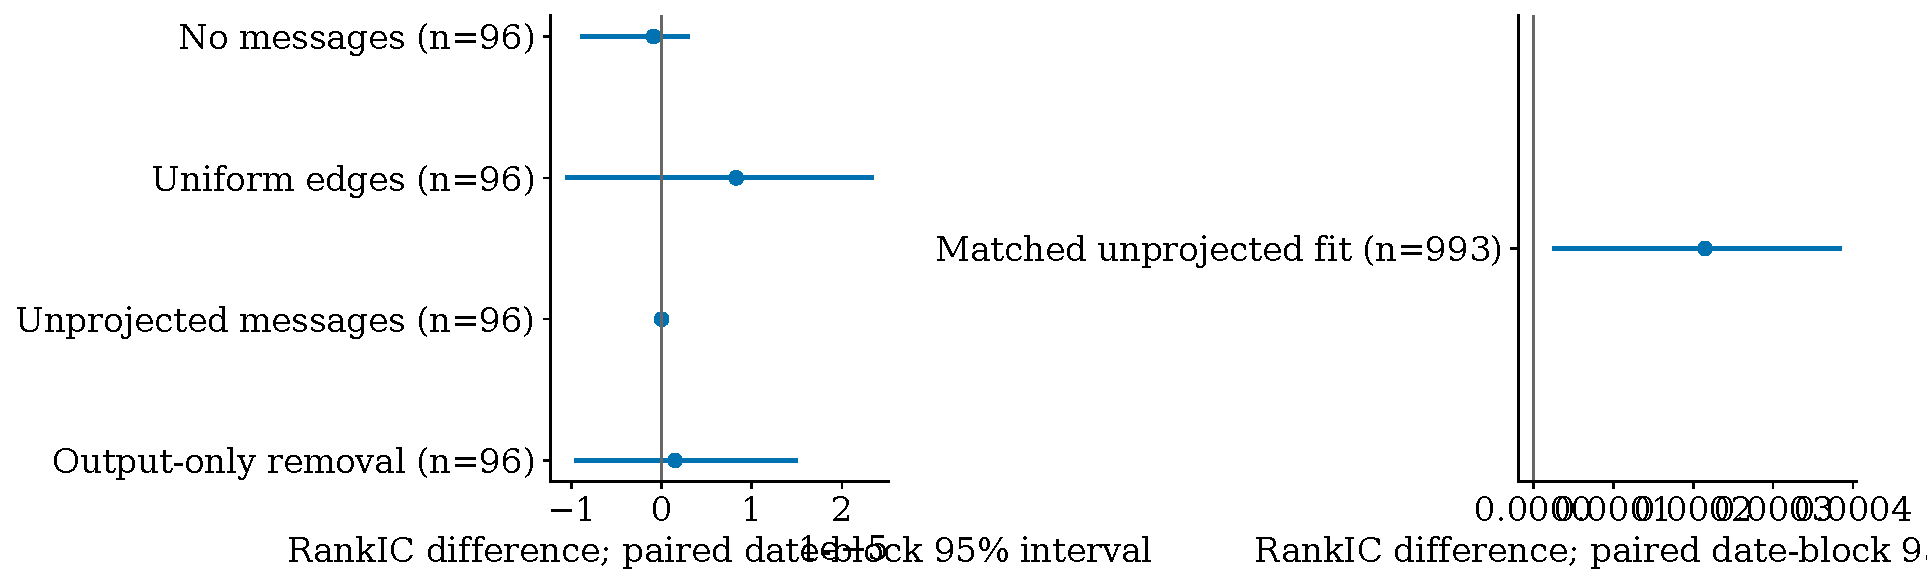
\includegraphics[width=.48\textwidth]{c3r_sp500_message_interventions.pdf}\hfill
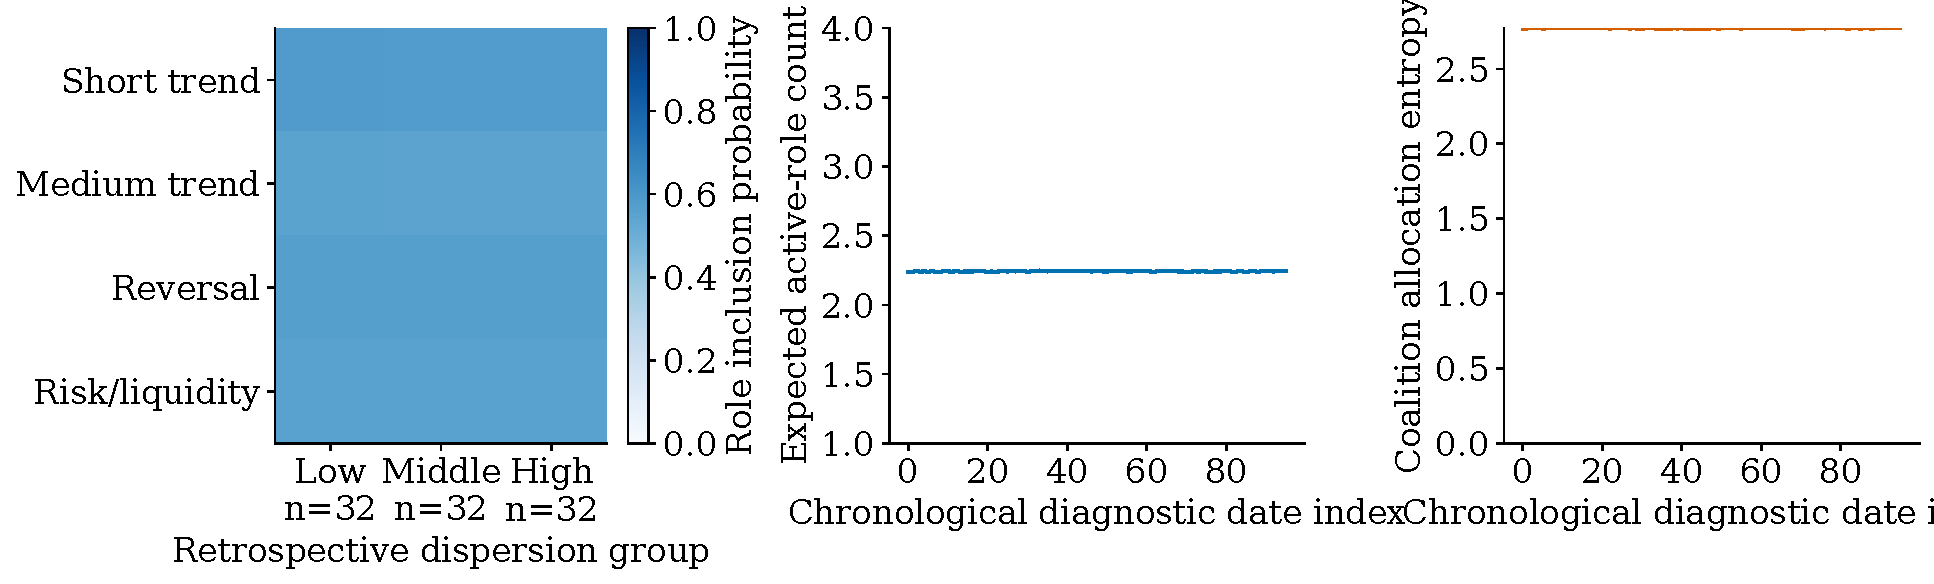
\includegraphics[width=.48\textwidth]{c3r_sp500_routing_behavior.pdf}
\caption{C3R activation on SP500. Left: message interventions and their paired RankIC changes. Right: coalition inclusion, expected active roles, and allocation entropy. The high-entropy, weakly differentiated route is consistent with compressed candidate-risk targets.}
\end{figure}

\begin{figure}[H]\centering
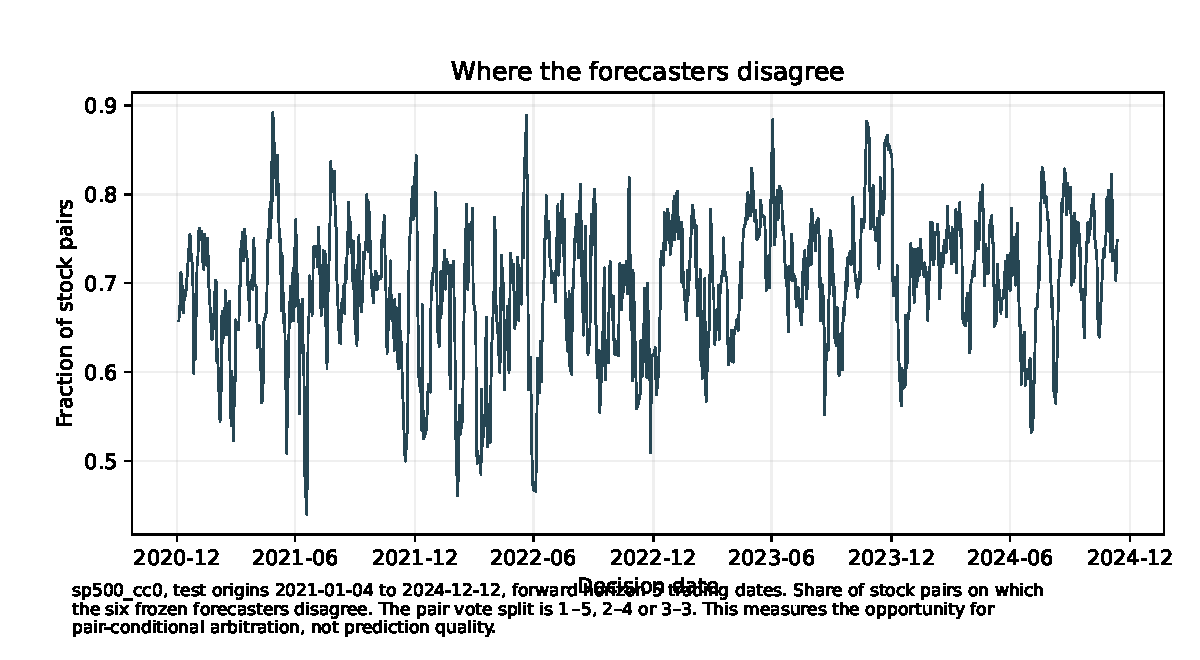
\includegraphics[width=.48\textwidth]{darc_sp500_disagreement.pdf}\hfill
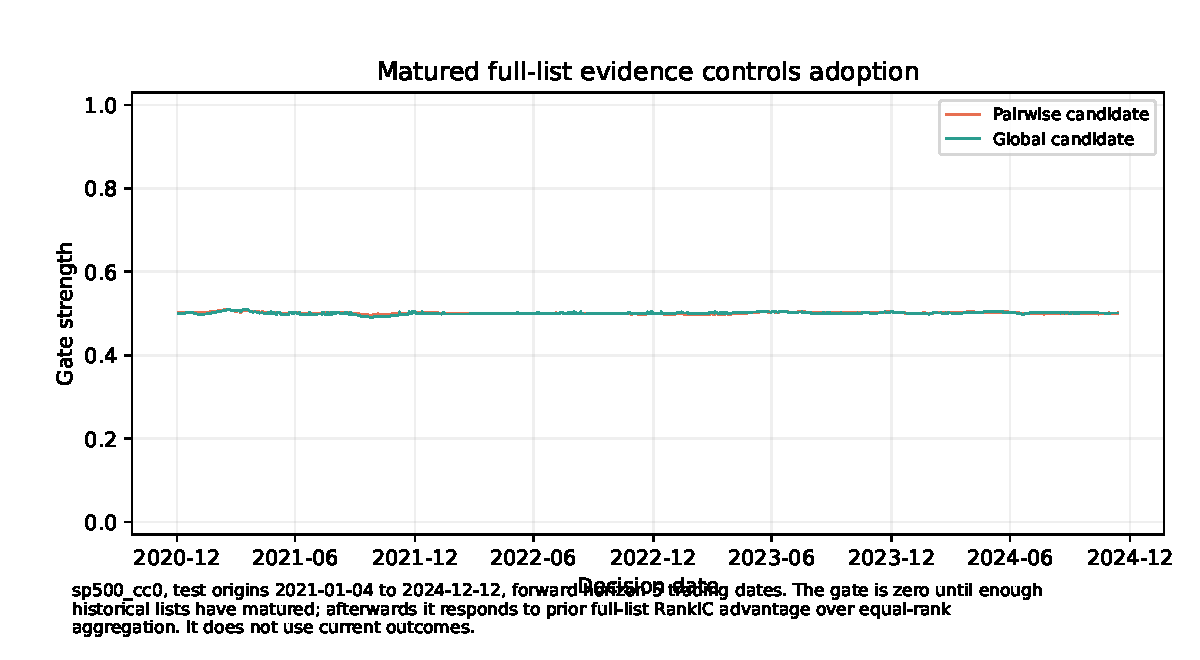
\includegraphics[width=.48\textwidth]{darc_sp500_gates.pdf}
\caption{DARC activation on SP500. Forecast disagreement creates opportunities for arbitration (left), while pairwise and global gate strength remain close to one half after the full history matures (right). Gate operation alone does not establish better final rankings.}
\end{figure}

\begin{figure}[H]\centering
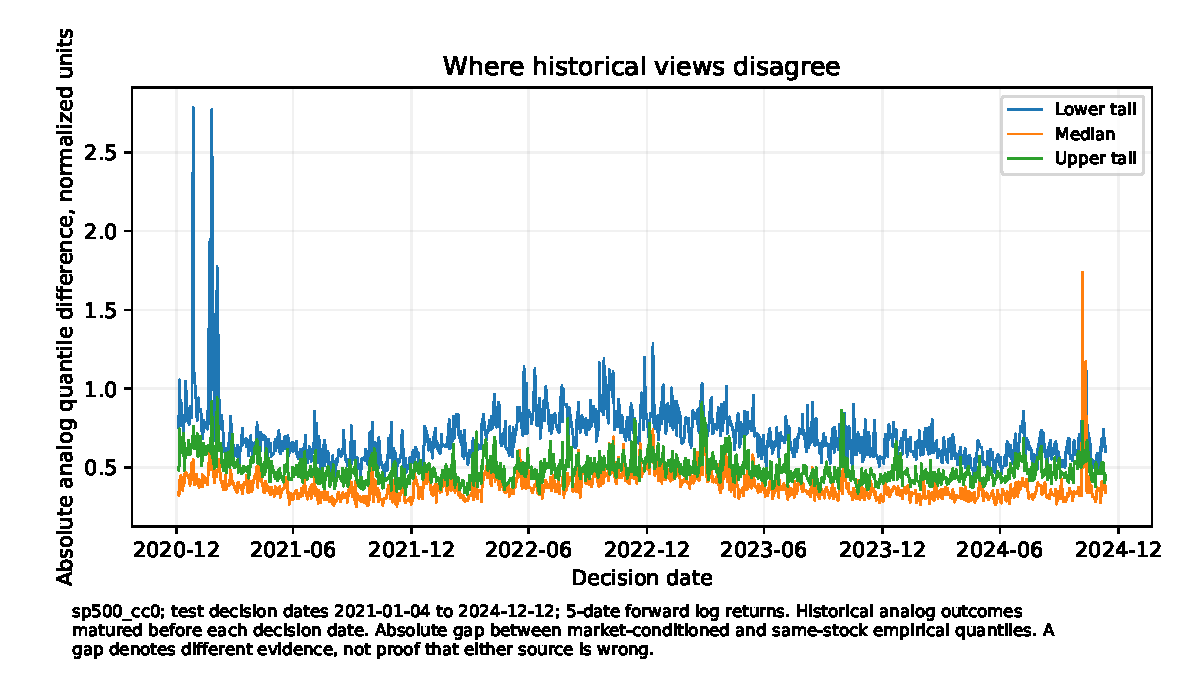
\includegraphics[width=.48\textwidth]{care_sp500_memory_disagreement.pdf}\hfill
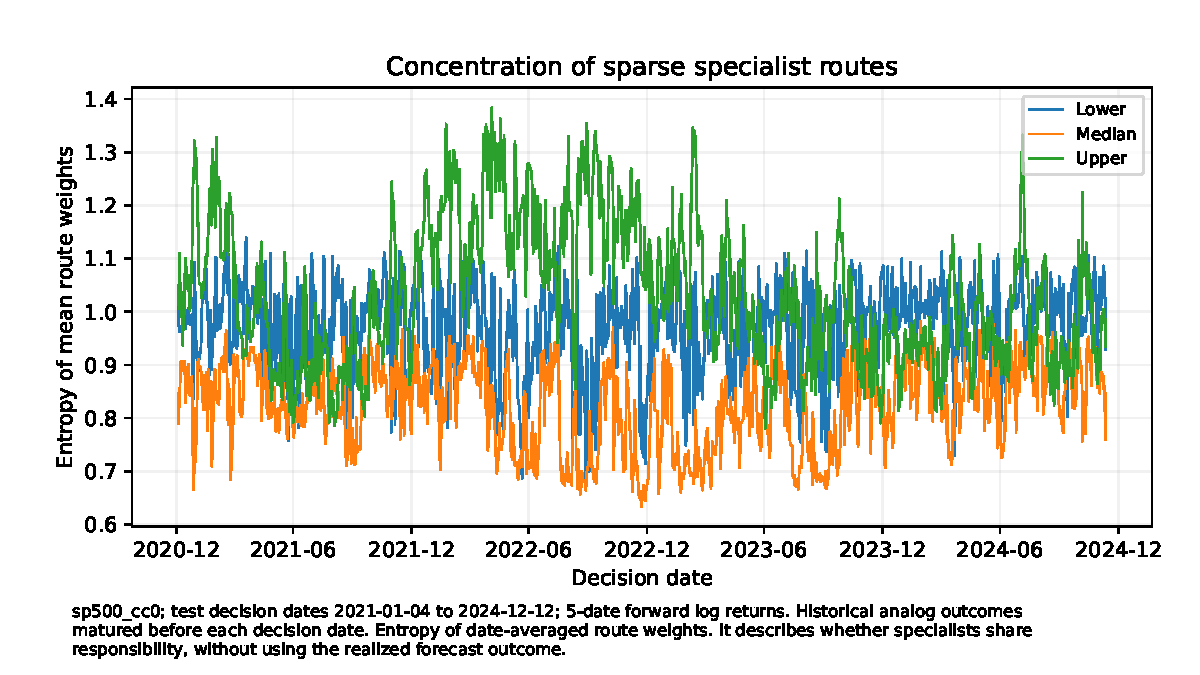
\includegraphics[width=.48\textwidth]{care_sp500_route_entropy.pdf}
\caption{CARE activation on SP500. Stock-specific and market memories disagree by a time-varying amount across quantiles (left), and specialist-route concentration also changes through time (right). The plots establish differentiated retrieval and routing, not lower pinball loss.}
\end{figure}

\begin{figure}[H]\centering
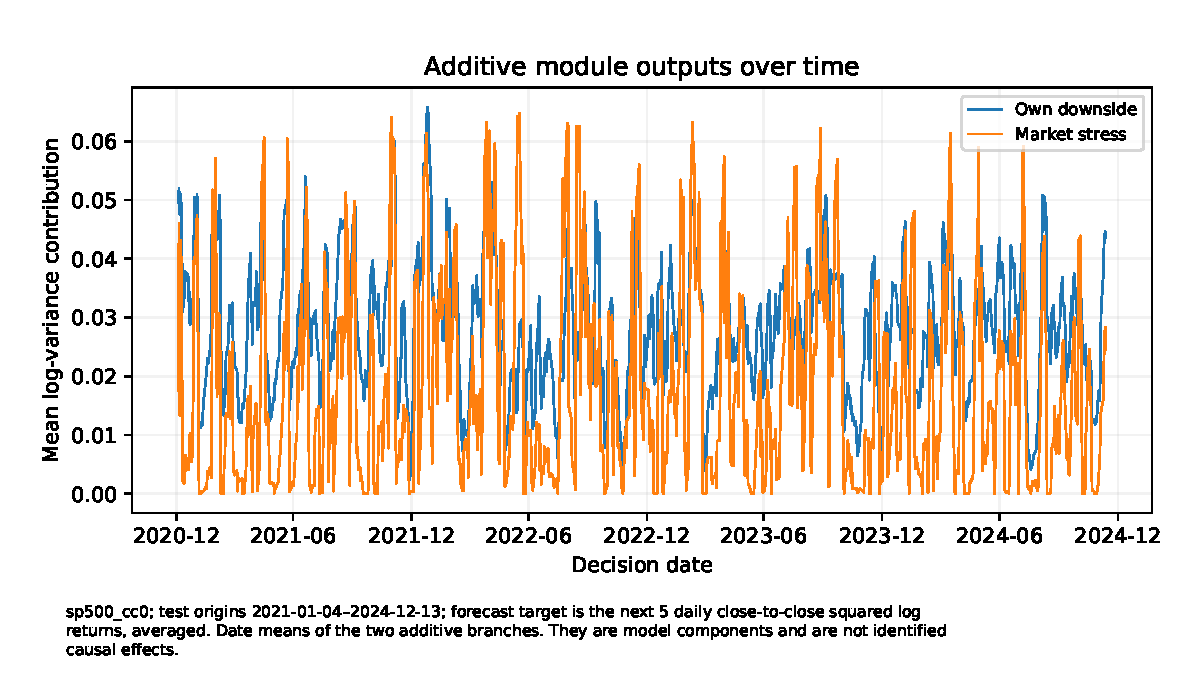
\includegraphics[width=.48\textwidth]{mosaic_sp500_branches.pdf}\hfill
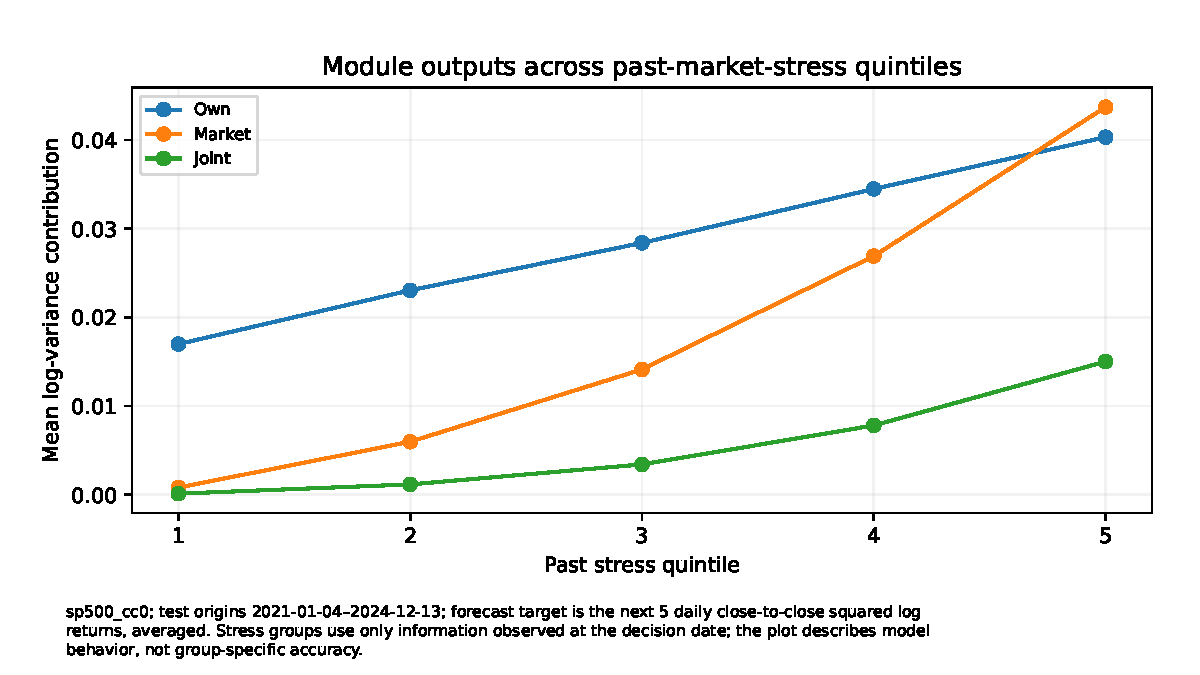
\includegraphics[width=.48\textwidth]{mosaic_sp500_stress.pdf}
\caption{MOSAIC activation on SP500. Both additive correction branches contribute over time (left), and the branch outputs increase across past-stress quintiles in the intended direction (right). These model-behavior diagnostics remain separate from external QLIKE comparisons.}
\end{figure}

\begin{figure}[H]\centering
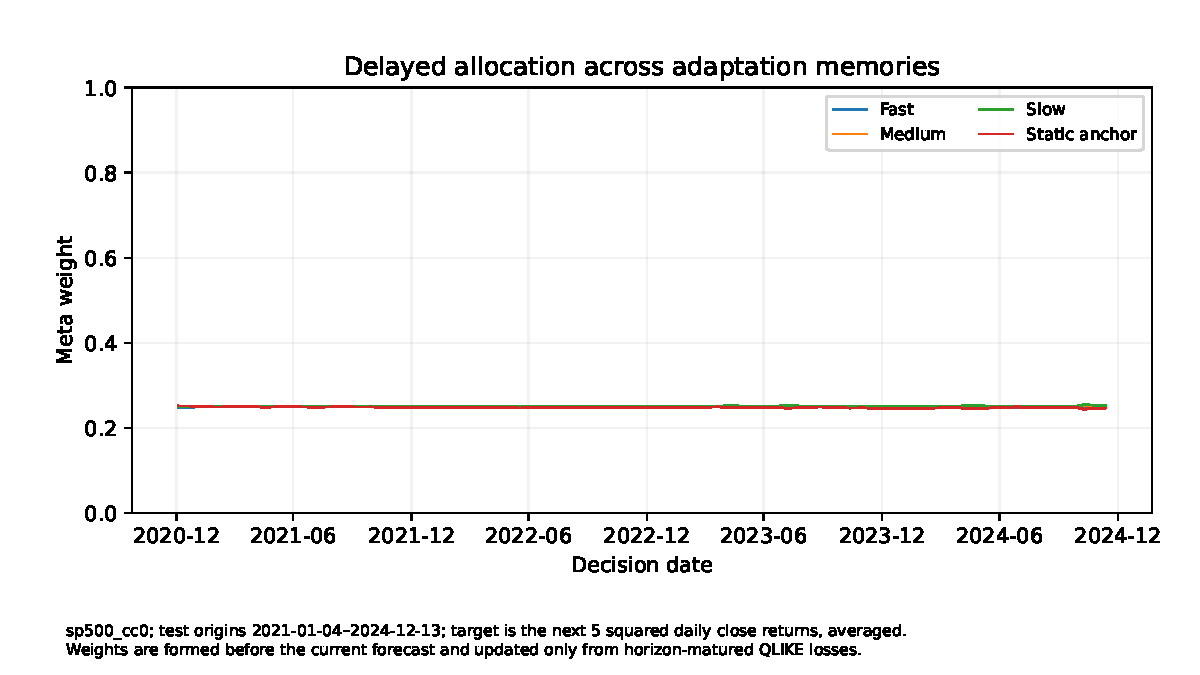
\includegraphics[width=.48\textwidth]{dashv_sp500_memory_weights.pdf}\hfill
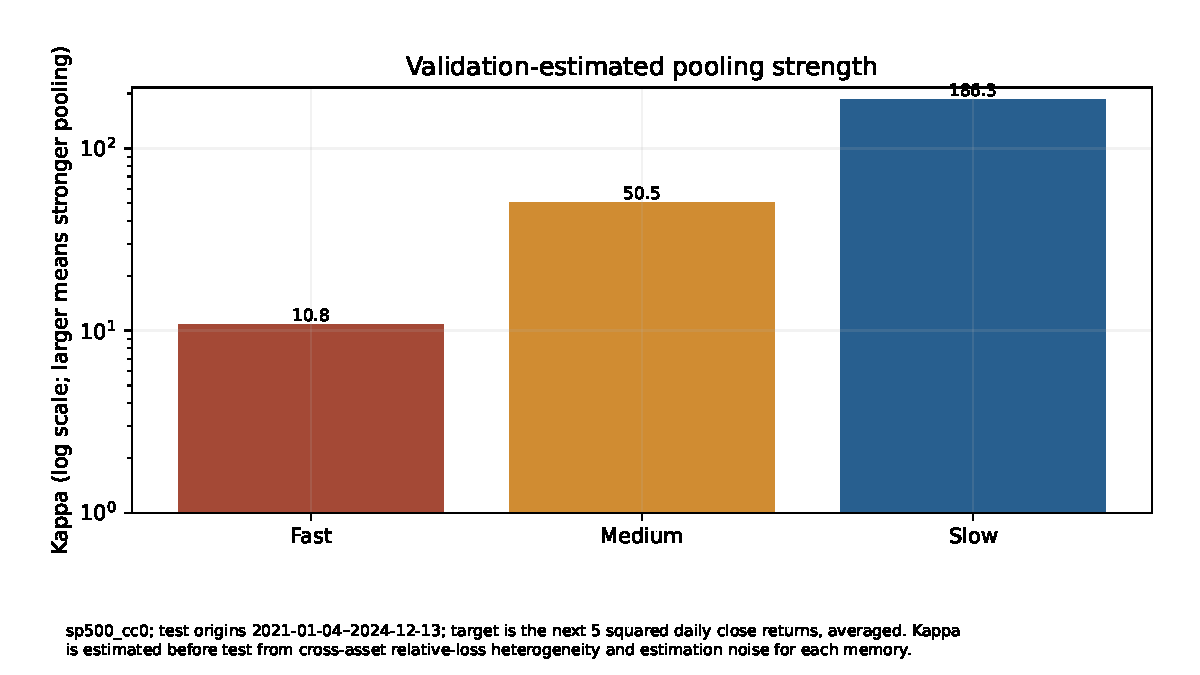
\includegraphics[width=.48\textwidth]{dashv_sp500_pooling_strength.pdf}
\caption{DASH-V activation on SP500. Delayed allocation across fast, medium, slow, and static memories stays close to equal weights (left), while validation-estimated pooling grows with memory scale (right). The hierarchy operates, but adaptive differentiation is limited.}
\end{figure}

\section{Factorial atlas}

\begin{figure}[H]\centering
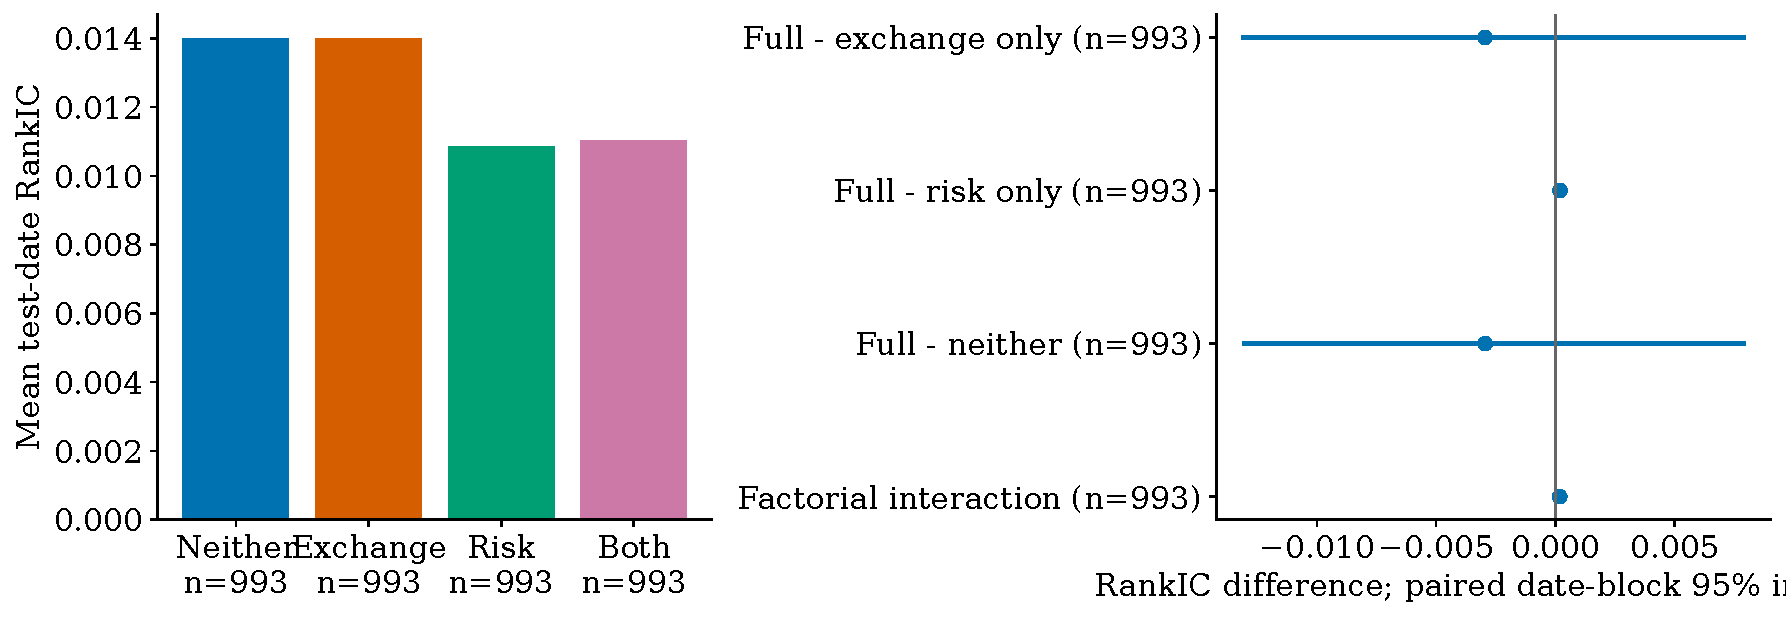
\includegraphics[width=.48\textwidth]{c3r_sp500_factorial.pdf}\hfill
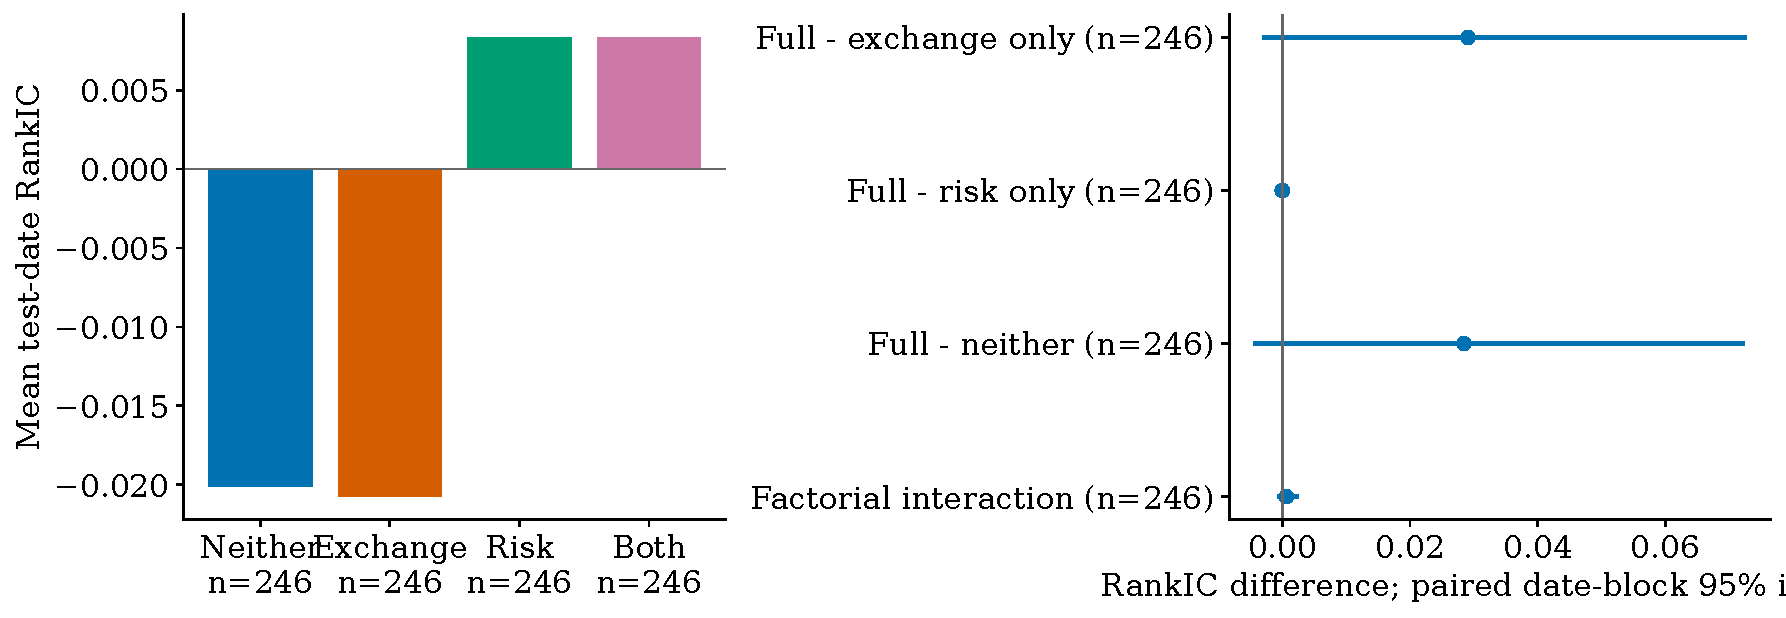
\includegraphics[width=.48\textwidth]{c3r_kdd17_factorial.pdf}\par\medskip
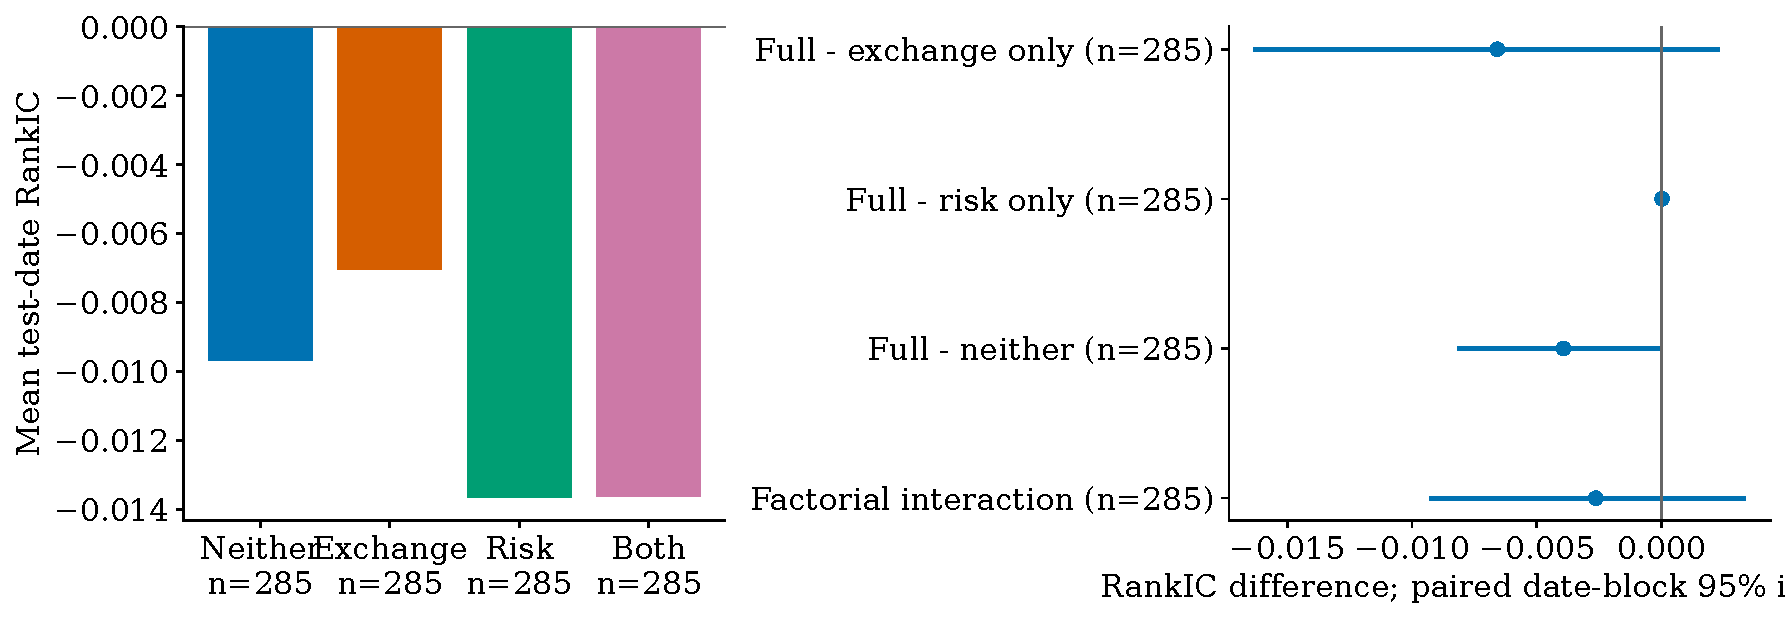
\includegraphics[width=.48\textwidth]{c3r_acl18_factorial.pdf}
\caption{C3R factorial cells on SP500, KDD17, and ACL18. The full model's favorable KDD17 point estimate is not accompanied by interval evidence and is largely reproduced by the risk-only cell.}
\end{figure}

\begin{figure}[H]\centering
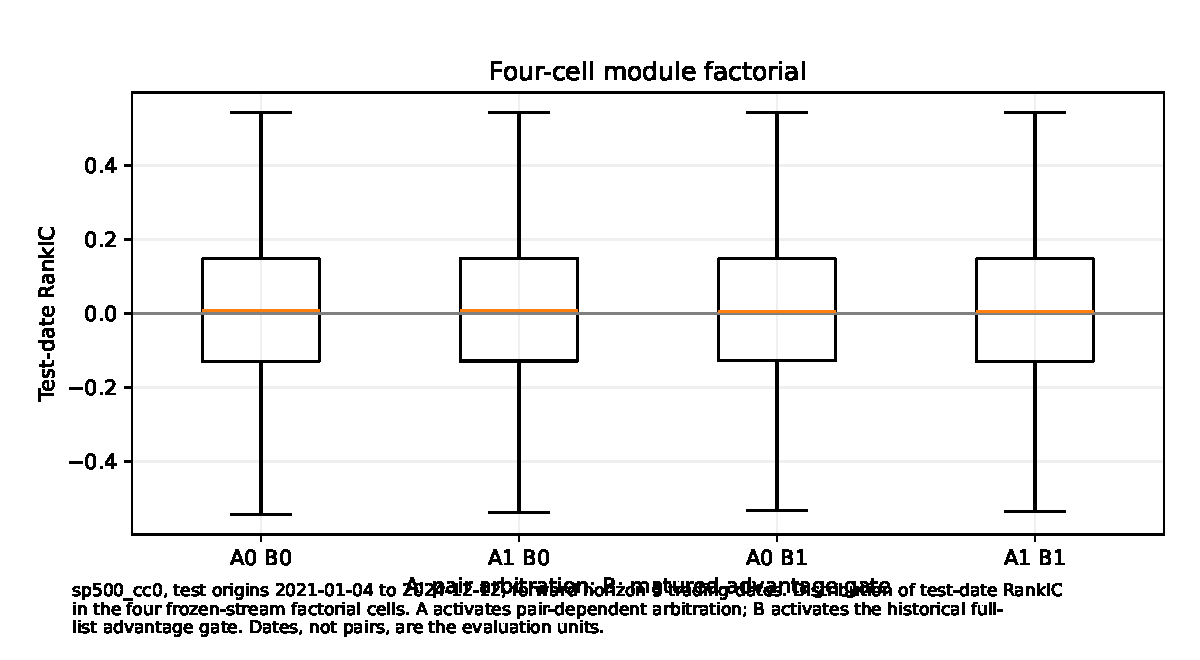
\includegraphics[width=.48\textwidth]{darc_sp500_factorial.pdf}\hfill
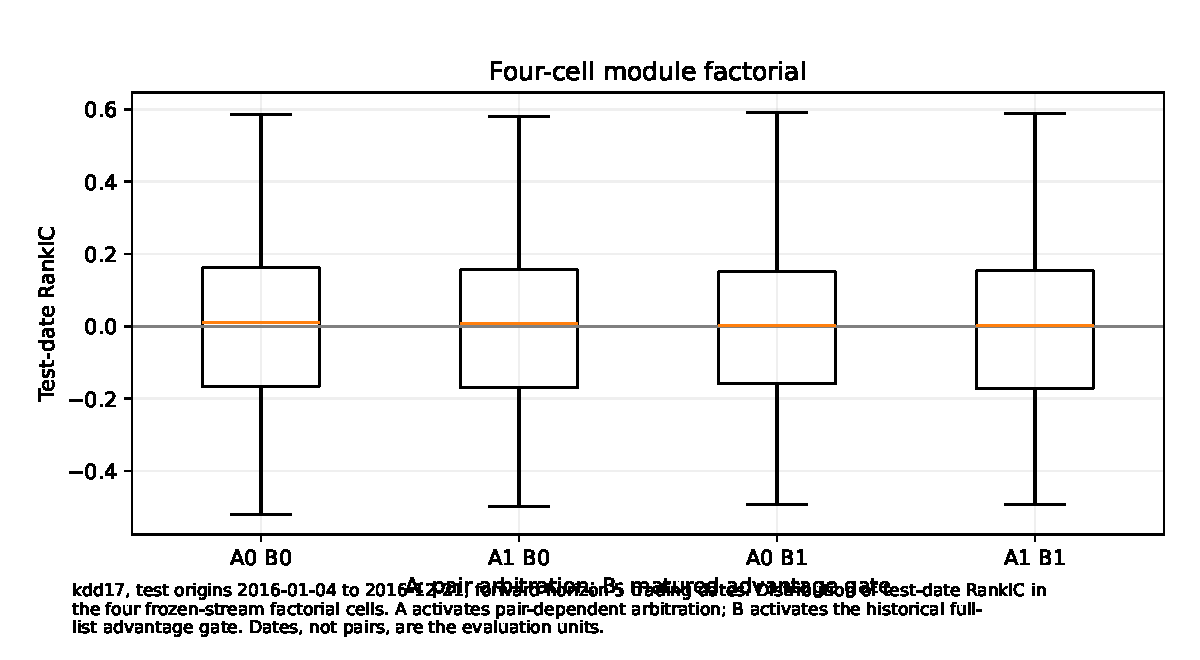
\includegraphics[width=.48\textwidth]{darc_kdd17_factorial.pdf}\par\medskip
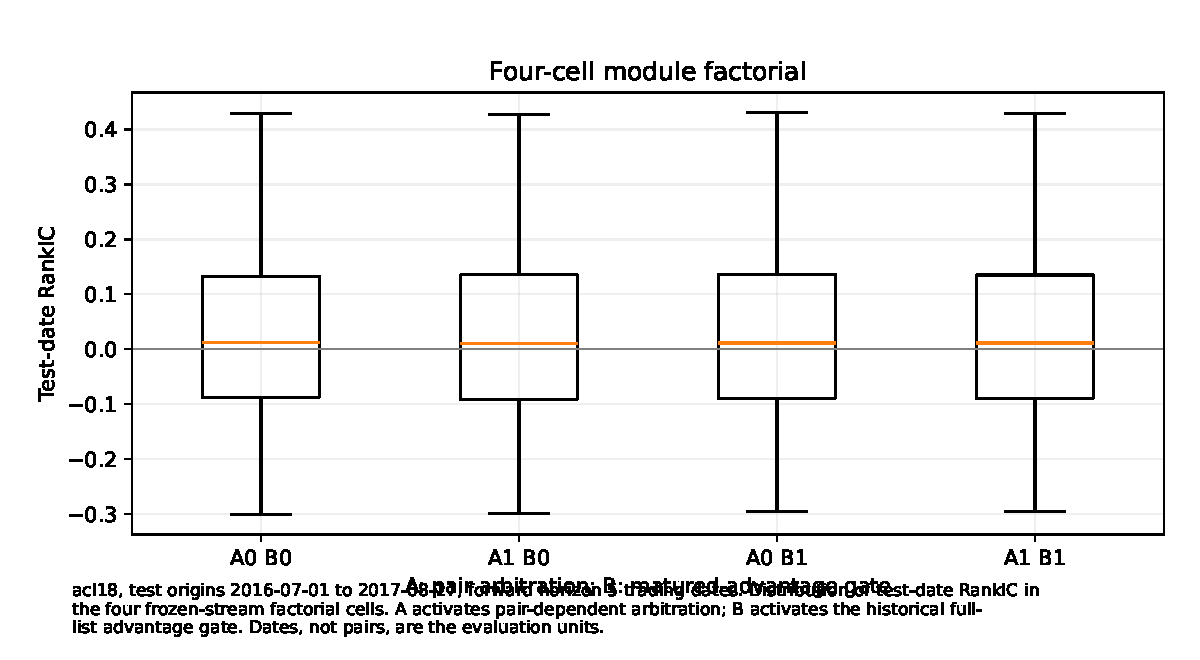
\includegraphics[width=.48\textwidth]{darc_acl18_factorial.pdf}
\caption{DARC factorial cells on the three panels. Pair-specific arbitration and the matured-advantage gate do not produce a supported interaction.}
\end{figure}

\begin{figure}[H]\centering
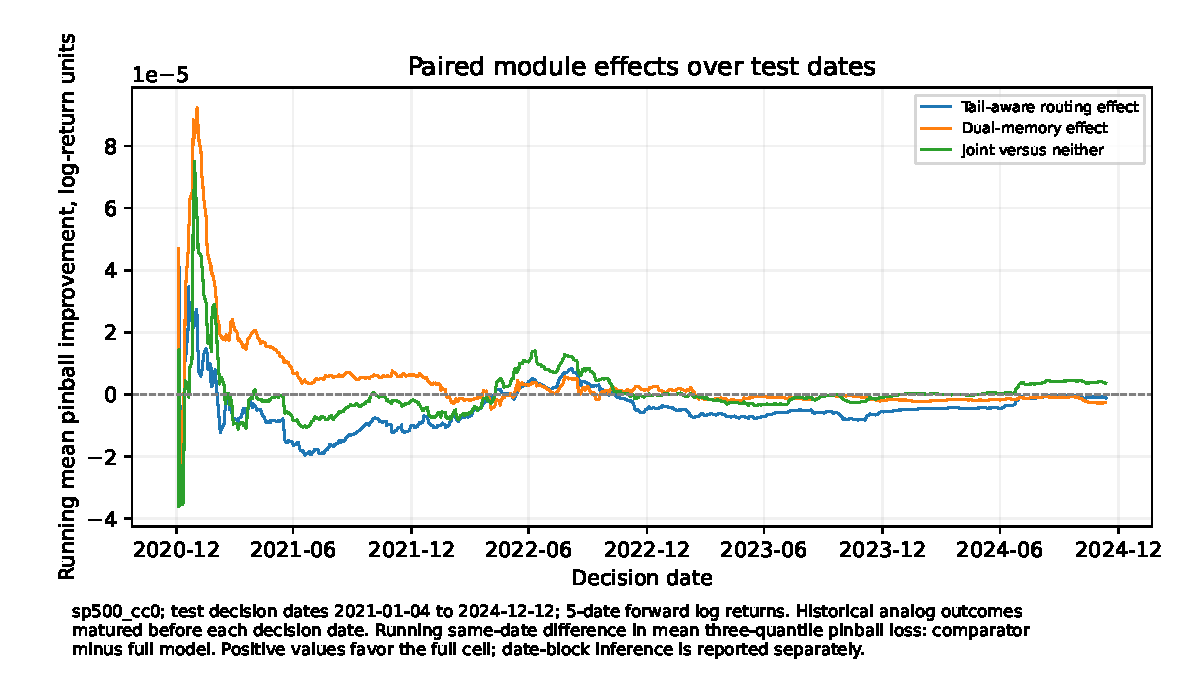
\includegraphics[width=.48\textwidth]{care_sp500_factorial.pdf}\hfill
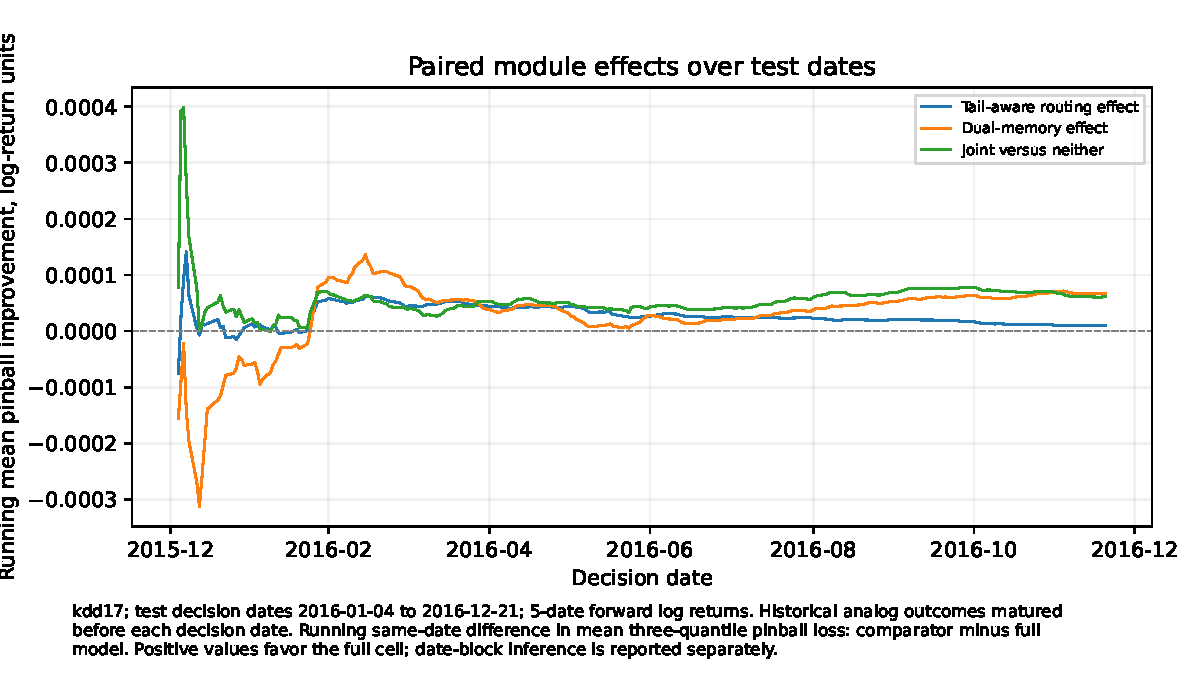
\includegraphics[width=.48\textwidth]{care_kdd17_factorial.pdf}\par\medskip
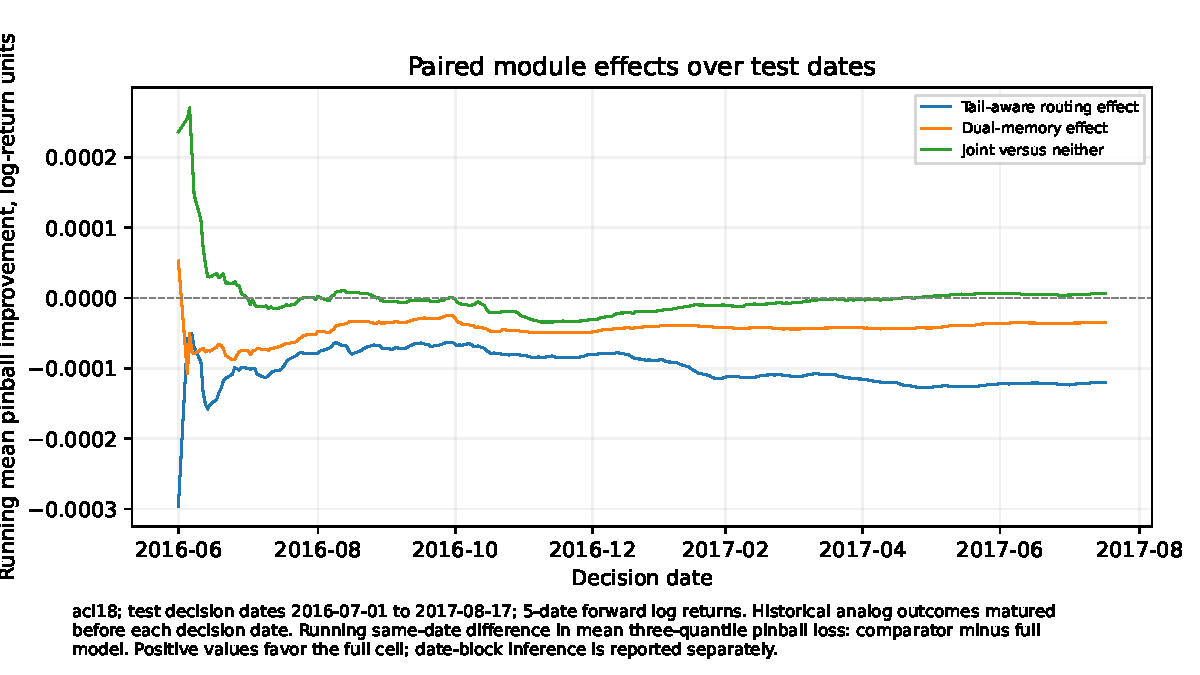
\includegraphics[width=.48\textwidth]{care_acl18_factorial.pdf}
\caption{CARE dual-memory by tail-routing factorial. The full cell is competitive but not the best pinball-loss model on any panel.}
\end{figure}

\begin{figure}[H]\centering
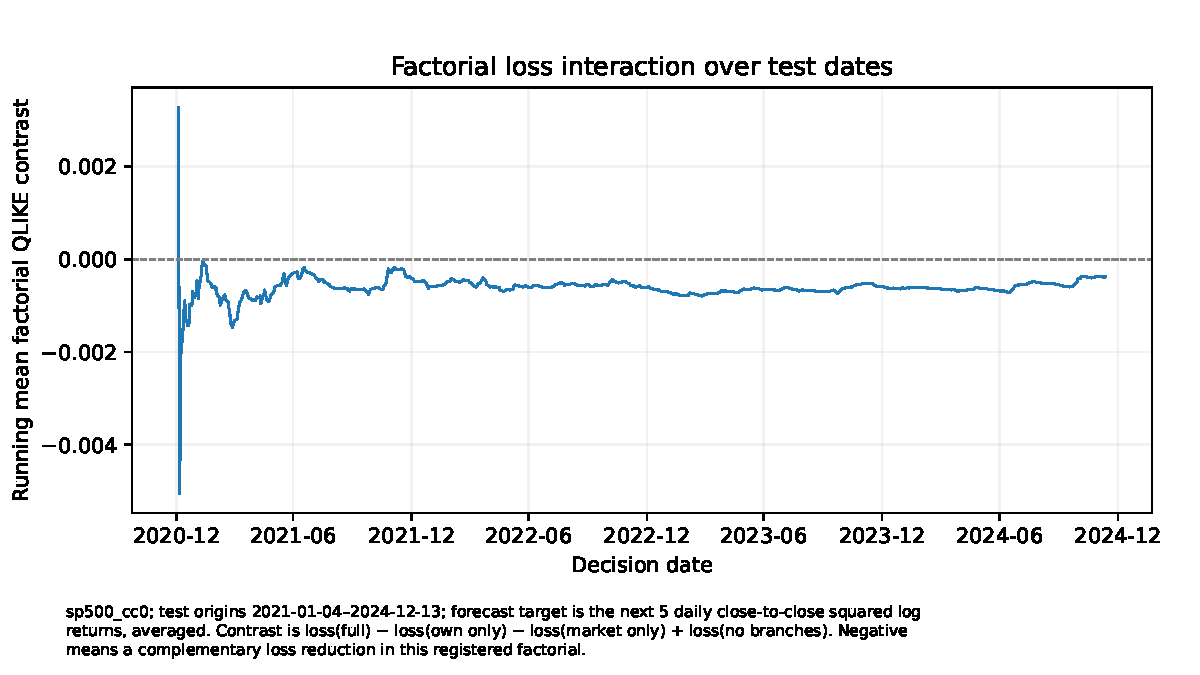
\includegraphics[width=.48\textwidth]{mosaic_sp500_factorial.pdf}\hfill
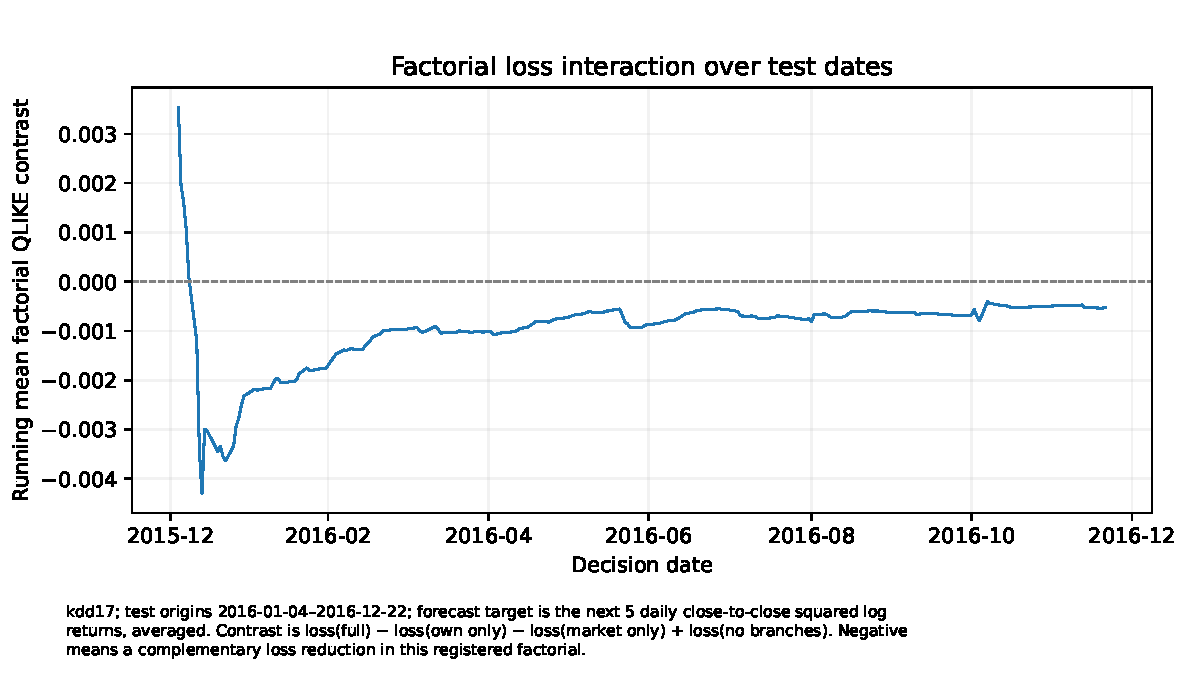
\includegraphics[width=.48\textwidth]{mosaic_kdd17_factorial.pdf}\par\medskip
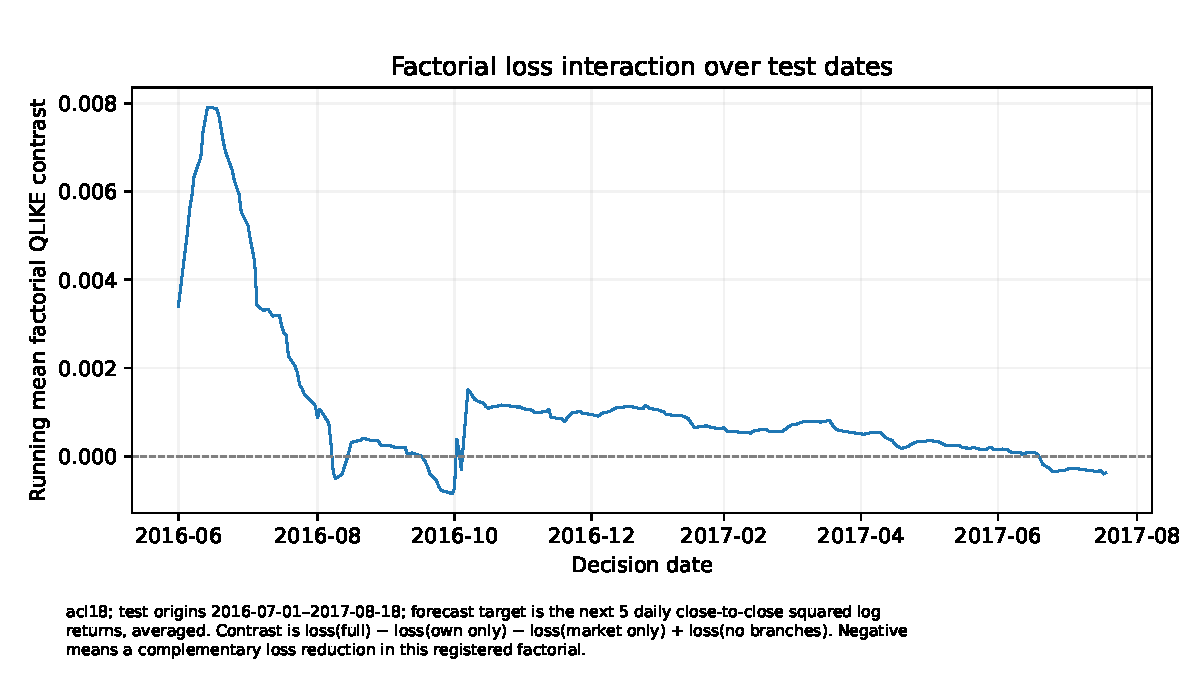
\includegraphics[width=.48\textwidth]{mosaic_acl18_factorial.pdf}
\caption{MOSAIC correction-branch factorial. Full-versus-base improvement is clearest on SP500, while the interaction intervals do not establish complementarity.}
\end{figure}

\begin{figure}[H]\centering
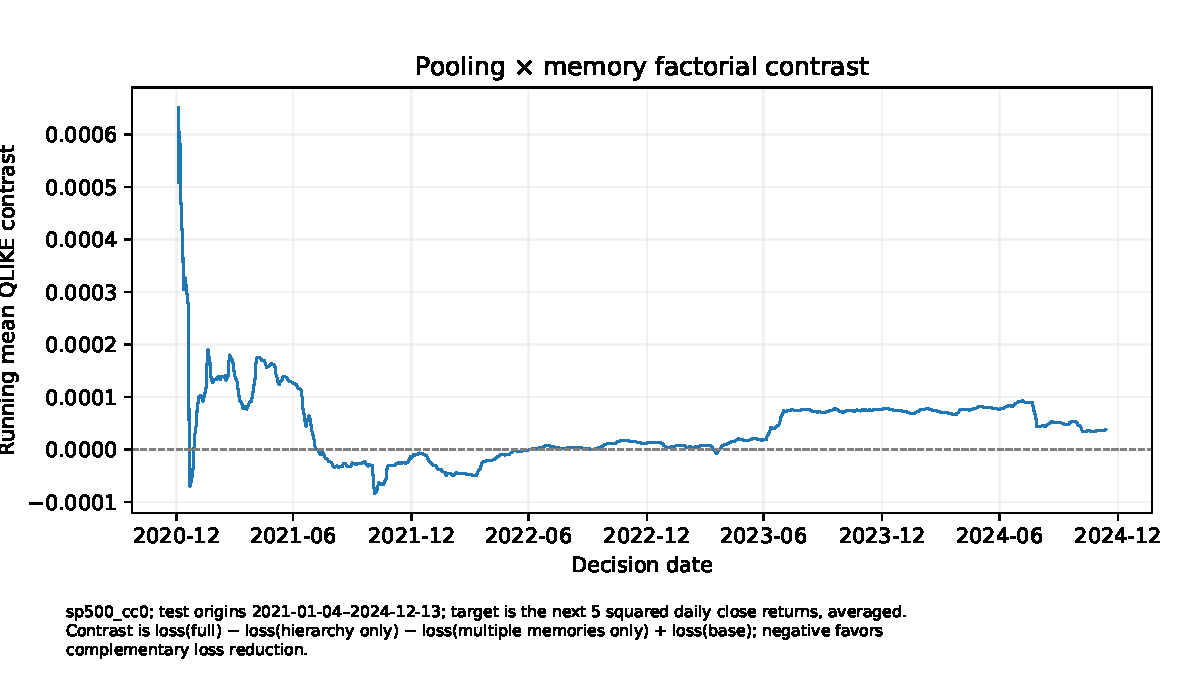
\includegraphics[width=.48\textwidth]{dashv_sp500_factorial.pdf}\hfill
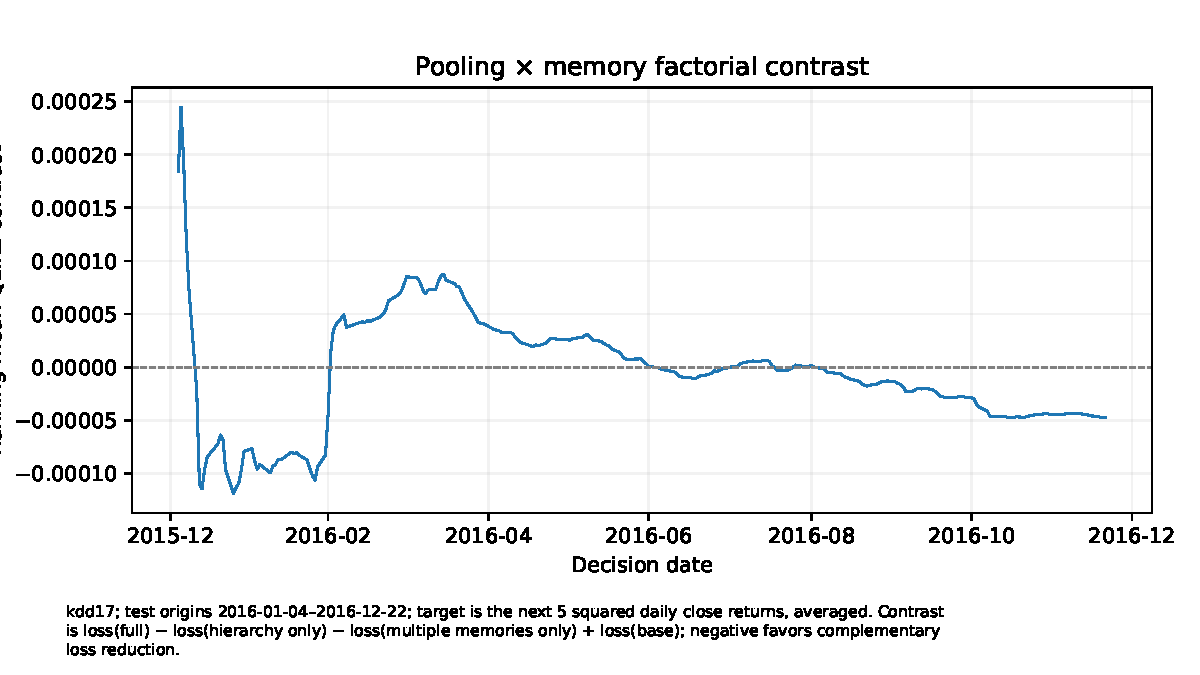
\includegraphics[width=.48\textwidth]{dashv_kdd17_factorial.pdf}\par\medskip
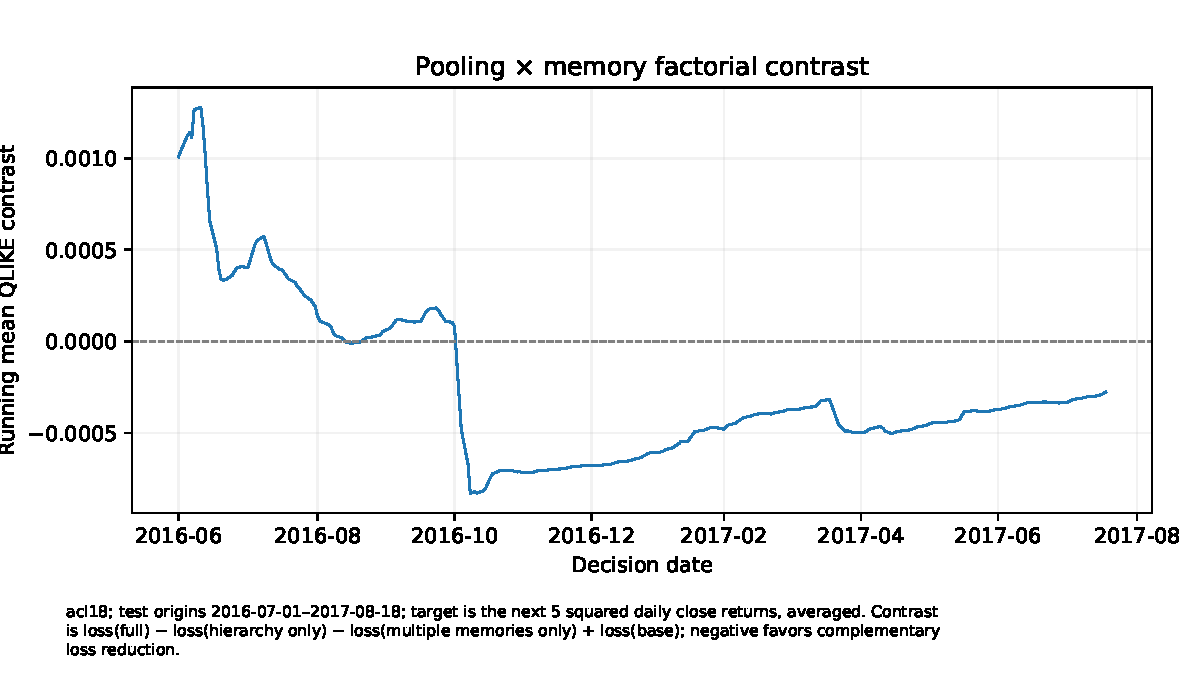
\includegraphics[width=.48\textwidth]{dashv_acl18_factorial.pdf}
\caption{DASH-V hierarchy by multiple-memory factorial. None of the interaction intervals supports the proposed complementarity.}
\end{figure}

\section{Interpretation rules}

The atlas is included to make module behavior inspectable. A non-flat route, changing weight, or nonzero correction establishes activation only. Incremental value requires a common-date comparison with the matched reduction. Broad value additionally requires a strong external comparator and consistent evidence across panels. Empty, failed, mixed, and adverse outcomes remain in the underlying archives.

The complete archive contains 120 vector PDF mechanism figures, eight per dataset for each study. Including every plot in the article would obscure the primary comparisons. The supplement therefore shows 25 panels: ten representative activation diagnostics on SP500 and fifteen factorial panels covering every study--dataset pair. The accompanying figure manifest maps every remaining file to its study and dataset, preserves its byte size and hash, and makes the selection auditable.

\end{document}
